\chapter{モンテカルロシミュレーションにおける実験評価(担当:水越)}\label{simulation}

この章では,実験が適切に構築されていることをモンテカルロシミュレーションを用いて評価する.
また,期待されるスペクトルを推定する.

\section{モンテカルロシミュレーションの意義}

本実験では,モンテカルロシミュレーションとしてGeant4\cite{geant4}を用いてプラスチックシンチレータの中で停止せずに陽電子がターゲットに到達し,ターゲットから発生したガンマ線がNaI(Tl)シンチレータで検出可能であることを確かめる.
また,実験でのバックグラウンドを推定する.

今回用いた線源は$\ce{^{22}Na}$ の標準線源であり,200 kBqのものである.
この線源強度と我々の実験期間が約1週間であることを考慮して,1 Hzの実験レートとS/N比100を目標に実験のデザインを検証した.


本章ではオルソポジトロニウムの寿命を測定する過程の評価を,$\ce{^{22}Na}$ 線源が$\beta$ 崩壊した陽電子がシンチレーターを通過してシリカゲルに到達する過程のレート評価(第\ref{section_test1}節),線源から直接NaI(Tl)シンチレータに入る$\gamma$ 線の評価(第\ref{section_test2}節),そして形成されたポジトロニウムが崩壊し,放出された$\gamma$ 線がNaI(Tl)シンチレータで落とすエネルギーの評価(第\ref{section_test3}節)の3つに分割してシミュレーションを行った.
また,モンテカルロシミュレーションで明らかにすることが難しい問題については第\ref{section_other}節で議論した.
これらをまとめた議論を第\ref{section_testall}節に示す.

プログラムの実装の都合上,シミュレーション結果の取得物理量に関係の無い線源\ce{^{22}Na}の寿命のみ,すぐに崩壊するよう付属のライブラリを書き換えた.
シミュレーションは全てGeant4の開発者にとって保守されているReference physics lists, LBEを用いて行った.

\section{プラスチックシンチレーターの通過}
\label{section_test1}

\subsection{概要}
今回の実験で用いられたプラスチックシンチレータは0.15 mmの厚みのものである.
線源から放出される陽電子が,シンチレータ内で停止するとシリカゲルに到達せずポジトロニウムを形成することができない.
ポジトロニウムを形成するためには,陽電子が標準線源の0.1 mmの厚みのアルミ窓を通過,空気中を伝播し,プラスチックシンチレータでエネルギーを落としきること無く通過する必要がある.
実際の線源を忠実に再現したジオメトリを作成し,シンチレータと線源の距離を変えながら通過してくる粒子の割合を調べた.



\subsection{ジオメトリ}

\begin{figure}[htbp]
	\centering
		\includegraphics[width=10cm]{img/test1_geometry.pdf}
	\caption{構築したジオメトリ}
	\label{test1_geometry}
\end{figure}

図\ref{test1_geometry} はプラスチックシンチレーターの試験として作成したジオメトリで,標準線源とその表面から距離$d$ mm離れたターゲットである直径8 mm,厚み0.15 mmのプラスチックシンチレーター(赤),その直後に置かれた理想的な粒子検出器で構成されている.
標準線源はアイソトープ協会のデータシートにしたがって作成し,アクリルのケースと0.1 mm厚のアルミニウム製の窓を実装した.
線源から向かってプラスチックシンチレータの裏側に実装した入射した理想的な検出器は,粒子の種類とエネルギーが分解能の影響を受けることなく検出可能な仮想的な検出器である.

ポジトロニウムにミキシングを起こすための磁場の方向を,プラスチックシンチレータまで誘導する方向に設定する.
陽電子が磁場方向に引き寄せられることが予想されるので,磁場の有無で実験レートを比較する.

図\ref{test1_geometry}では事象例として\ce{^{22}Na}が100 個崩壊した軌跡を表示している.
非常に多くの緑の線で示されているのが$\gamma$線,青の線で示されているのが陽電子の軌跡である.

\subsection{陽電子到達数と立体角}

プラスチックシンチレーターと線源間の距離の増加にしたがって,通過してくる陽電子数は減少すると考えられる.
この減少には,空気中を伝播する際に陽電子が相互作用することも影響すると考えられるが,大部分の影響は立体角の減少に由来すると予想される.
立体角$\Omega$\,srは解析的に計算すると,

\begin{equation}
	\nonumber
	\Omega = 2\pi \left( 1-\cos\left(\arctan\frac{8.0/2}{d+2.5}\right)\right)
\end{equation}

で与えられる.今回は$d$を線源の表面からシンチレーターを通過するまでの距離と定義しているので,放射線源中心からの補正2.5 mmを加えている.

\subsection{結果と考察}

図\ref{test1}は$d=100$\,mmで,$10^8$事象生成した際のシンチレーターを通過した陽電子のエネルギースペクトル(青)である. シンチレーターを外したとき(赤)と比較した.

また,図\ref{scinti_test}がシンチレーターを陽電子が通過する割合の距離依存である.磁場をかけたとき(赤)とかけていないとき(青)をプロットし,$d=10$\, mmの点と重なるように規格化した立体角を重ね書きした(緑).


\begin{figure}[htbp]
	\centering
		\includegraphics[width=10cm]{fig/test1.pdf}
	\caption{シンチレータを透過した陽電子のエネルギー}
	\label{test1}
\end{figure}


\begin{figure}[htbp]
	\centering
		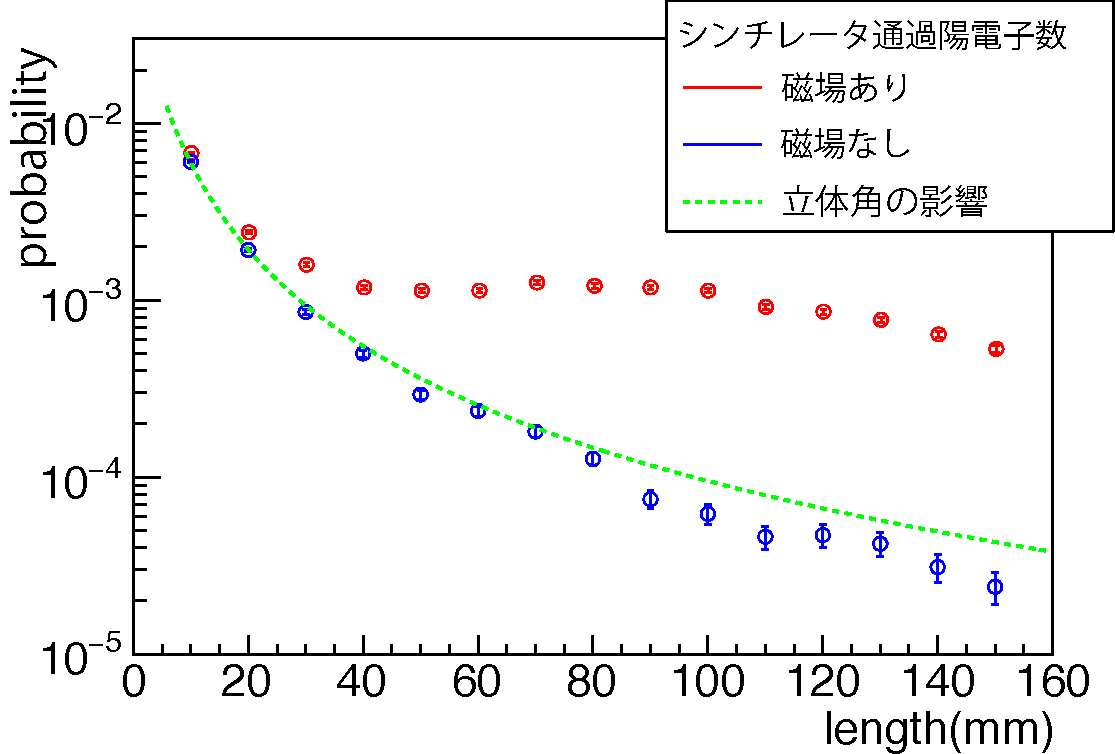
\includegraphics[width=10cm]{fig/scinti_test.pdf}
	\caption{プラスチックシンチレータ通過粒子割合}
	\label{scinti_test}
\end{figure}


図\ref{test1}より, プラスチックシンチレータでおよそ40\%程度陽電子を損失するが,$\beta$崩壊に対し約1/1000の陽電子が到達し実験に十分な陽電子が通過していると判断する.

%一方で,磁場をかけたときとかけていないときで,陽電子の到達数には差がある,
図\ref{scinti_test}では,磁場の無いときは陽電子数は距離が伸びるにつれてほぼ立体角に従い減り続けていくが,磁場のある際には40--110 mm程度まで陽電子数に大きな変化がない.
磁場なしの結果で$d$が大きいとき立体角の影響よりやや陽電子数が少なくなることは空気中でのエネルギー損失によるものと考えられる.
この結果より実際の設計ではターゲットであるシリカゲルまで100 mm程度線源から離した.

\subsection{鉛コリメータの実装}
この章のまとめとして,実際の実験に近いジオメトリで,陽電子がシンチレータを通過する確率を評価する.
ジオメトリの可視化より,$\gamma$線バックグラウンドが非常に多くなる事が予想される.
線源から出る$\gamma$線が直接NaI(Tl)シンチレータで検出されることを防ぐため,鉛のコリメータを実装する.

\begin{figure}[htbp]
	\centering
		\includegraphics[width=10cm]{img/test1b_geometry.pdf}
	\caption{実装した鉛コリメータ}
	\label{test1b_geometry}
\end{figure}

\begin{figure}[htbp]
	\centering
		\includegraphics[width=10cm]{fig/collimator_loss.pdf}
	\caption{鉛コリメータで失われる陽電子}
	\label{collimator_loss}
\end{figure}

図\ref{test1b_geometry}は鉛のコリメータを実装した様子である.先の考察から線源までの距離を100 mmとし,そこに鉛のコリメータをおいた.NaI(Tl)シンチレータをできる限りターゲットに近づけて立体角を大きくすることを考えるため,鉛のコリメータは72 mmの幅,高さと奥行きを100 mmで設計した.また,直径16 mmの穴をターゲットに向けてあけた.NaIシンチレータの配置されるターゲット側に到達する$\gamma$線の数は大きく減少している.

図\ref{collimator_loss}は鉛のコリメータをおいたとき(赤)と置かないとき(青)の到達する陽電子数の比較である.
大きなバックグラウンドの減少と同時に,事象数も鉛コリメータの壁面に陽電子が衝突することで減少すると考えられる.

この事象数の減少に対するバックグラウンド事象数の減少割合は,第\ref{section_test2}節で評価する.

本モンテカルロシミュレーションでは,線源での$\beta$崩壊$10^7$事象中,13,550事象がプラスチックシンチレータを通過してシリカゲルに到達した.



\section{線源からのバックグラウンド評価}
\label{section_test2}

\subsection{概要}
第\ref{section_test1}節のプラスチックシンチレータの評価で,ターゲットのシリカゲルに到達する陽電子数を定量的に見積った.
本節ではポジトロニウム生成事象に対して,バックグラウンドとなる線源から放出される$\gamma$線が.NaIシンチレータで検出されるバックグラウンドの量を定量的に評価する.


\subsection{ジオメトリ}
実際の実験装置とほとんど同じジオメトリを構築し,シミュレーションを行った.図\ref{test2_geometry}が構築したジオメトリである.赤で示されているものが今回の実験のターゲットであるシリカゲルであり,線源側の窓には\ref{section_test1}節のシミュレーションで用いたものと同じプラスチックシンチレータが実装されている.線源は鉛のコリメータで覆われ,青で陽電子の軌跡が表示されている.シリカゲルはNaI(Tl)シンチレータで囲まれている.
線源が$\beta$崩壊し,NaI(Tl)シンチレータで$\gamma$線がエネルギーを落とす事象を記録する.陽電子がシリカゲル中でエネルギーを失い,対消滅によって発生した$\gamma$線がNaI(Tl)シンチレータでとらえられる事象に対して,線源からの$\gamma$線が直接NaI(Tl)シンチレータで検出される事象をバックグラウンドとしてエネルギースペクトルを求めた.

\begin{figure}[htbp]
	\centering
		
\includegraphics[width=10cm]{img/test2_geometry.pdf}
	\caption{構築したジオメトリ}
	\label{test2_geometry}
\end{figure}

\subsection{結果と考察}

図\ref{test2}が$\beta$崩壊での事象とバックグラウンドのエネルギースペクトルである.

表\ref{table_test2}に,鉛コリメータの有無による,NaI(Tl)シンチレータで検出される事象とバックグラウンドの事象数を示す.
線源の$\beta$崩壊$10^8$事象に対して,バックグラウンドが127,455事象NaIシンチレータで検出される.


\begin{figure}[htbp]
	\centering
		\includegraphics[width=10cm]{fig/test2.pdf}
	\caption{トリガーを考慮しない事象とバックグラウンド}
	\label{test2}
\end{figure}

\begin{table}[htbp]
	\centering
	\caption{鉛コリメータの有無による事象数}
		\label{table_test2}	
	  \begin{tabular}{ccc} 
		\hline
		   				&事象& バックグラウンド \\ 
		\hline \hline
		鉛コリメータなし & 20,865 & 1,007,762 \\
		鉛コリメータあり & 1,419  & 127,455   \\
		\hline
	  \end{tabular}
\end{table}

図\ref{test2bXY},図\ref{test2bYZ}に陽電子がエネルギーを失い停止したシリカゲル中での位置を示す.
図\ref{test2bXY}の横軸はシリカゲルの表面を示し,縦軸方向で停止位置の深さを示している.
この深さ方向をX軸とし,図\ref{test2bYZ}では直径8 mmのシンチレータ中のでの停止Y--Z位置を示している.

\begin{figure}[htbp]
	\centering
		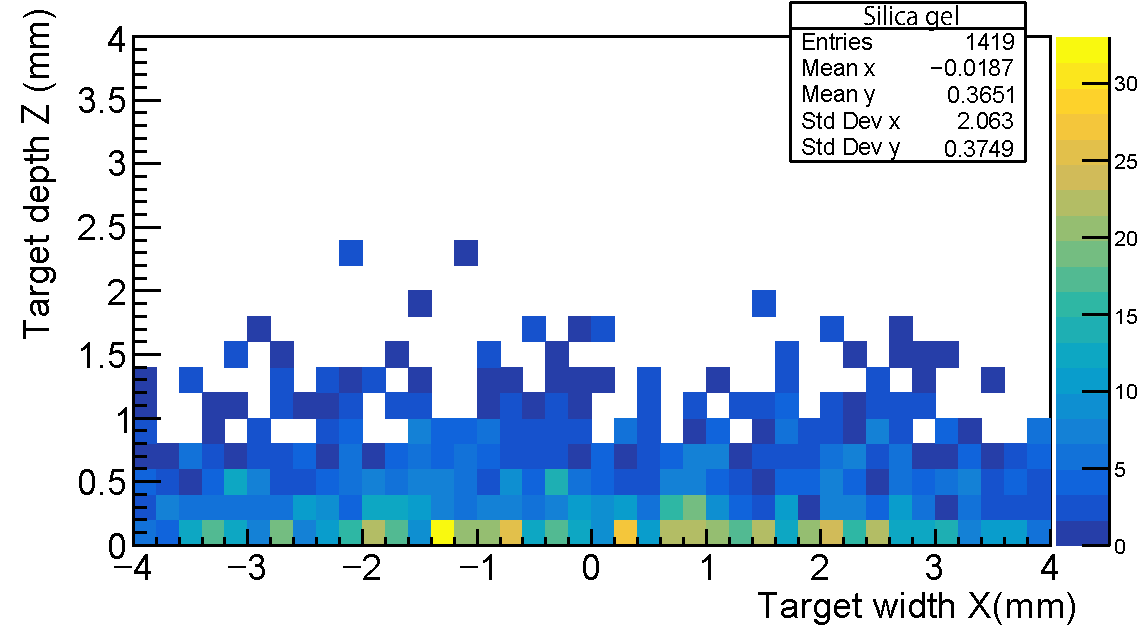
\includegraphics[width=10cm]{fig/test2bXY.pdf}
	\caption{陽電子停止位置深さX-Y方向}
	\label{test2bXY}
\end{figure}

\begin{figure}[htbp]
	\centering
		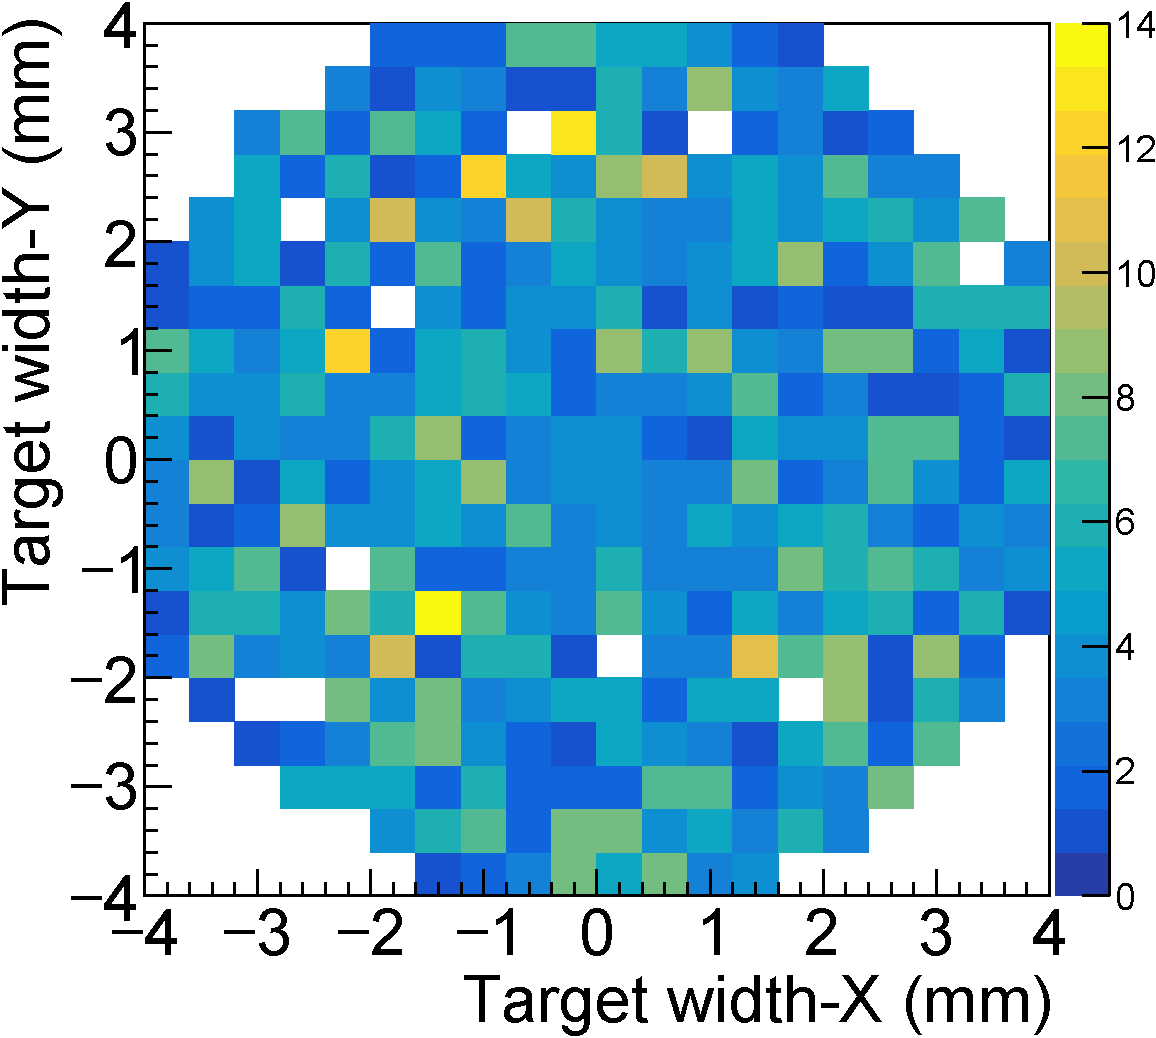
\includegraphics[width=7cm]{fig/test2bYZ.pdf}
	\caption{陽電子停止位置Y-Z方向}
	\label{test2bYZ}
\end{figure}


図\ref{test2}は\ce{^{22}Na}の崩壊に対するエネルギースペクトルを示している.バックグラウンド事象が非常に多いが,プラスチックシンチレータを用いたトリガーを用いてアクシデンタル事象を除くバックグラウンドのほとんどを落とすことができると期待される.具体的な事象レートとアクシデンタル由来のバックグラウンドレートの値については全てのシミュレーションを踏まえて第\ref{section_testall}節で検討する.また,エネルギーによるカットをかけられることが同時に期待される.

表\ref{table_test2}で,鉛コリメータを置くことで事象数は7 \%程度になってしまうが,一方でバックグラウンド事象を1 \%近くまで低減可能である.
本実験において,鉛コリメータが有用であるということが示された.

図\ref{test2bXY}から陽電子はシリカエアロゲル中で,平均して0.3 mmの深さで停止し,2 mm以下でほぼ全ての陽電子が停止する.
シリカエアロゲルケースは15 mmの深さで設計されており,陽電子の貫通に対して十分に深いと考えられる.
図\ref{test2bYZ}ではシンチレータの大きさに対してほぼ均等に陽電子が到達していることがわかる.
設計の直径8 mmは薄いシンチレータの強度に由来する最大の値であるためこれ以上大きくすることはできず,シンチレータをこれ以上小さくすると事象数が減少する.


\section{予想されるエネルギースペクトル}
\label{section_test3}

\subsection{ポジトロニウムの崩壊}

先述の2つのシミュレーションにより,我々の実験での事象頻度が概算された.最後に,この実験によって実際にどのような物理量が得られるべきか検討する.
公式にリリースされているGeant4にはポジトロニウムの様なエキゾチック系の挙動は含まれておらず,前項でのシミュレーションでは陽電子はシリカゲル中で$2\gamma$崩壊していた.本項ではパラポジトロニウムとオルソポジトロニウムの崩壊を実装し,NaI(Tl)シンチレータで検出する確率とエネルギースペクトルを推定する.また,オルソポジトロニウムの$3\gamma$崩壊を検討し第\ref{section_test2}節で行った評価に補正を加える.

実際にはスピン交換反応や,ピックオフ反応が起こり,実際に入射した陽電子がオルソポジトロニウムを形成し,$3\gamma$に崩壊する確率の理論的な予測は不可能であるため,$2\gamma$に崩壊する事象と$3\gamma$に崩壊する事象を同数生成しシミュレーションを行う.

\subsection{結果と考察}

図\ref{gamma2}はパラポジトロニウムに典型的な$2\gamma$崩壊,図\ref{gamma3}はオルソポジトロニウムに典型的な$3\gamma$崩壊の期待される実験スペクトルである.
ここでは装置の分解能は考慮していない.

\begin{figure}[htbp]
	\begin{tabular}{cc}

	\centering
		\begin{minipage}{0.5\hsize}
		\includegraphics[width=7cm]{fig/gamma2.pdf}
	\caption{$2\gamma$崩壊のスペクトル}
	\label{gamma2}
		\end{minipage}&

		\begin{minipage}{0.5\hsize}
	\centering
		\includegraphics[width=7cm]{fig/gamma3.pdf}
	\caption{$3\gamma$崩壊のスペクトル}
	\label{gamma3}
		\end{minipage}

		\end{tabular}
\end{figure}

図\ref{gamma2}で示される2$\gamma$崩壊では電子と陽電子の質量に等しい511 keVの$\gamma$線が発生し,光電ピークとして現れている.
一方,図\ref{gamma3}で示される$3\gamma$崩壊では連続スペクトルが観測される.
本モンテカルロシミュレーションでは,陽電子がシリカエアロゲルに到達し,$3\gamma$崩壊を$10^7$事象が起こったとき,2,418,889個の$\gamma$線をNaIシンチレータで検出した.


\section{その他の物理量の概算}
\label{section_other}

\subsection{$3\gamma$崩壊事象と$2\gamma$崩壊事象との比の推定}
前述の様に$2\gamma$事象と$3\gamma$事象の比は理論で予測することはできない.
オルソポジトロニウムとパラポジトロニウムの生成比は3:1であるが,オルソポジトロニウムはスピン交換反応をおこしパラポジトロニウムに変わってしまう.
また,ポジトロニウム中の陽電子が周囲の原子分子中の電子と対消滅するピックオフ消滅も起こる.
ピックオフ消滅を減らすため,シリカエアロゲルを真空状態に保つ工夫をしているが,それでも完全に無視することはできない.
したがって定量的な予測を行うことは難しいため,昨年度の本研究室の卒業研究の結果などから$2\gamma$事象と$3\gamma$事象数が1:1であると見積もった.

\subsection{プラスチックシンチレータのトリガー効率}
陽電子,あるいは$\gamma$線がシンチレータでエネルギーを落とすことはモンテカルロシミュレーションで確かめることができる.
一方で,シンチレータの発光による光子の検出効率は見測定である.
このトリガー効率を10\%と見積もる.

\subsection{2$\gamma$事象由来のバックグラウンド}
すくないということをいう予定.

\subsection{宇宙線,自然放射線由来のバックグラウンド}
すくないということをいう予定.\cite{小早川201207}

\section{実験評価のまとめ}
\label{section_testall}

\subsection{実験レートとバックグラウンドの推定}
実験結果を統合し,実験レートを推定する.
推定される実験での事象レートは図\ref{test1}から予測されるシリカゲルへの陽電子の到達確率,プラスチックシンチレータのトリガー効率,$3\gamma$事象の比,図\ref{gamma3}で予測される$\gamma$線がNaI(Tl)シンチレータで検出される確率と,線源強度200 kBqの積として求められる.

\begin{equation}
	\nonumber
	\frac{13,550}{10 \mathrm{M}} \times \frac{10}{100} \times \frac{1}{2} \times \frac{2,418,889}{10 \mathrm{M}} \times 200 \mathrm{kBq} \sim 3.3 \mathrm{Hz}
\end{equation}
ゆえに事象レートは3.3 Hzと見積もられる.

図\ref{test2}からトリガーをかける前のバックグラウンド事象のレートを求めると,
\begin{equation}
	\nonumber
	\frac{127,455}{100\mathrm{M}} \times 200 \mathrm{kBq} \sim 250 \mathrm{ Hz}
\end{equation}
ゆえに,トリガーをかけても落としきれないアクシデンタル事象のレートは,トリガーでゲートを1$\si{\micro \second}$開くとすると,
\begin{equation}
	\nonumber
	( 1 \si{\micro \second} + 1 \si{\micro \second}) \times  250 \mathrm{Hz} \times 3.3 \mathrm{Hz} \sim 1.7 \times 10^{-3} \mathrm{Hz}
\end{equation}
であり,目標としていたレート1 Hz, S/N比100のデザインをみたしていると言える.図\ref{test_all}はこのレートで1週間の測定を行った際に期待されるスペクトルである.

\begin{figure}[htbp]
	\centering
		\includegraphics[width=10cm]{fig/test_all.pdf}
	\caption{1週間の測定で期待されるスペクトル(若干修正予定)}
	\label{test_all}
\end{figure}

